\begin{figure*}[t]
\centering
\resizebox{\textwidth}{!}{%
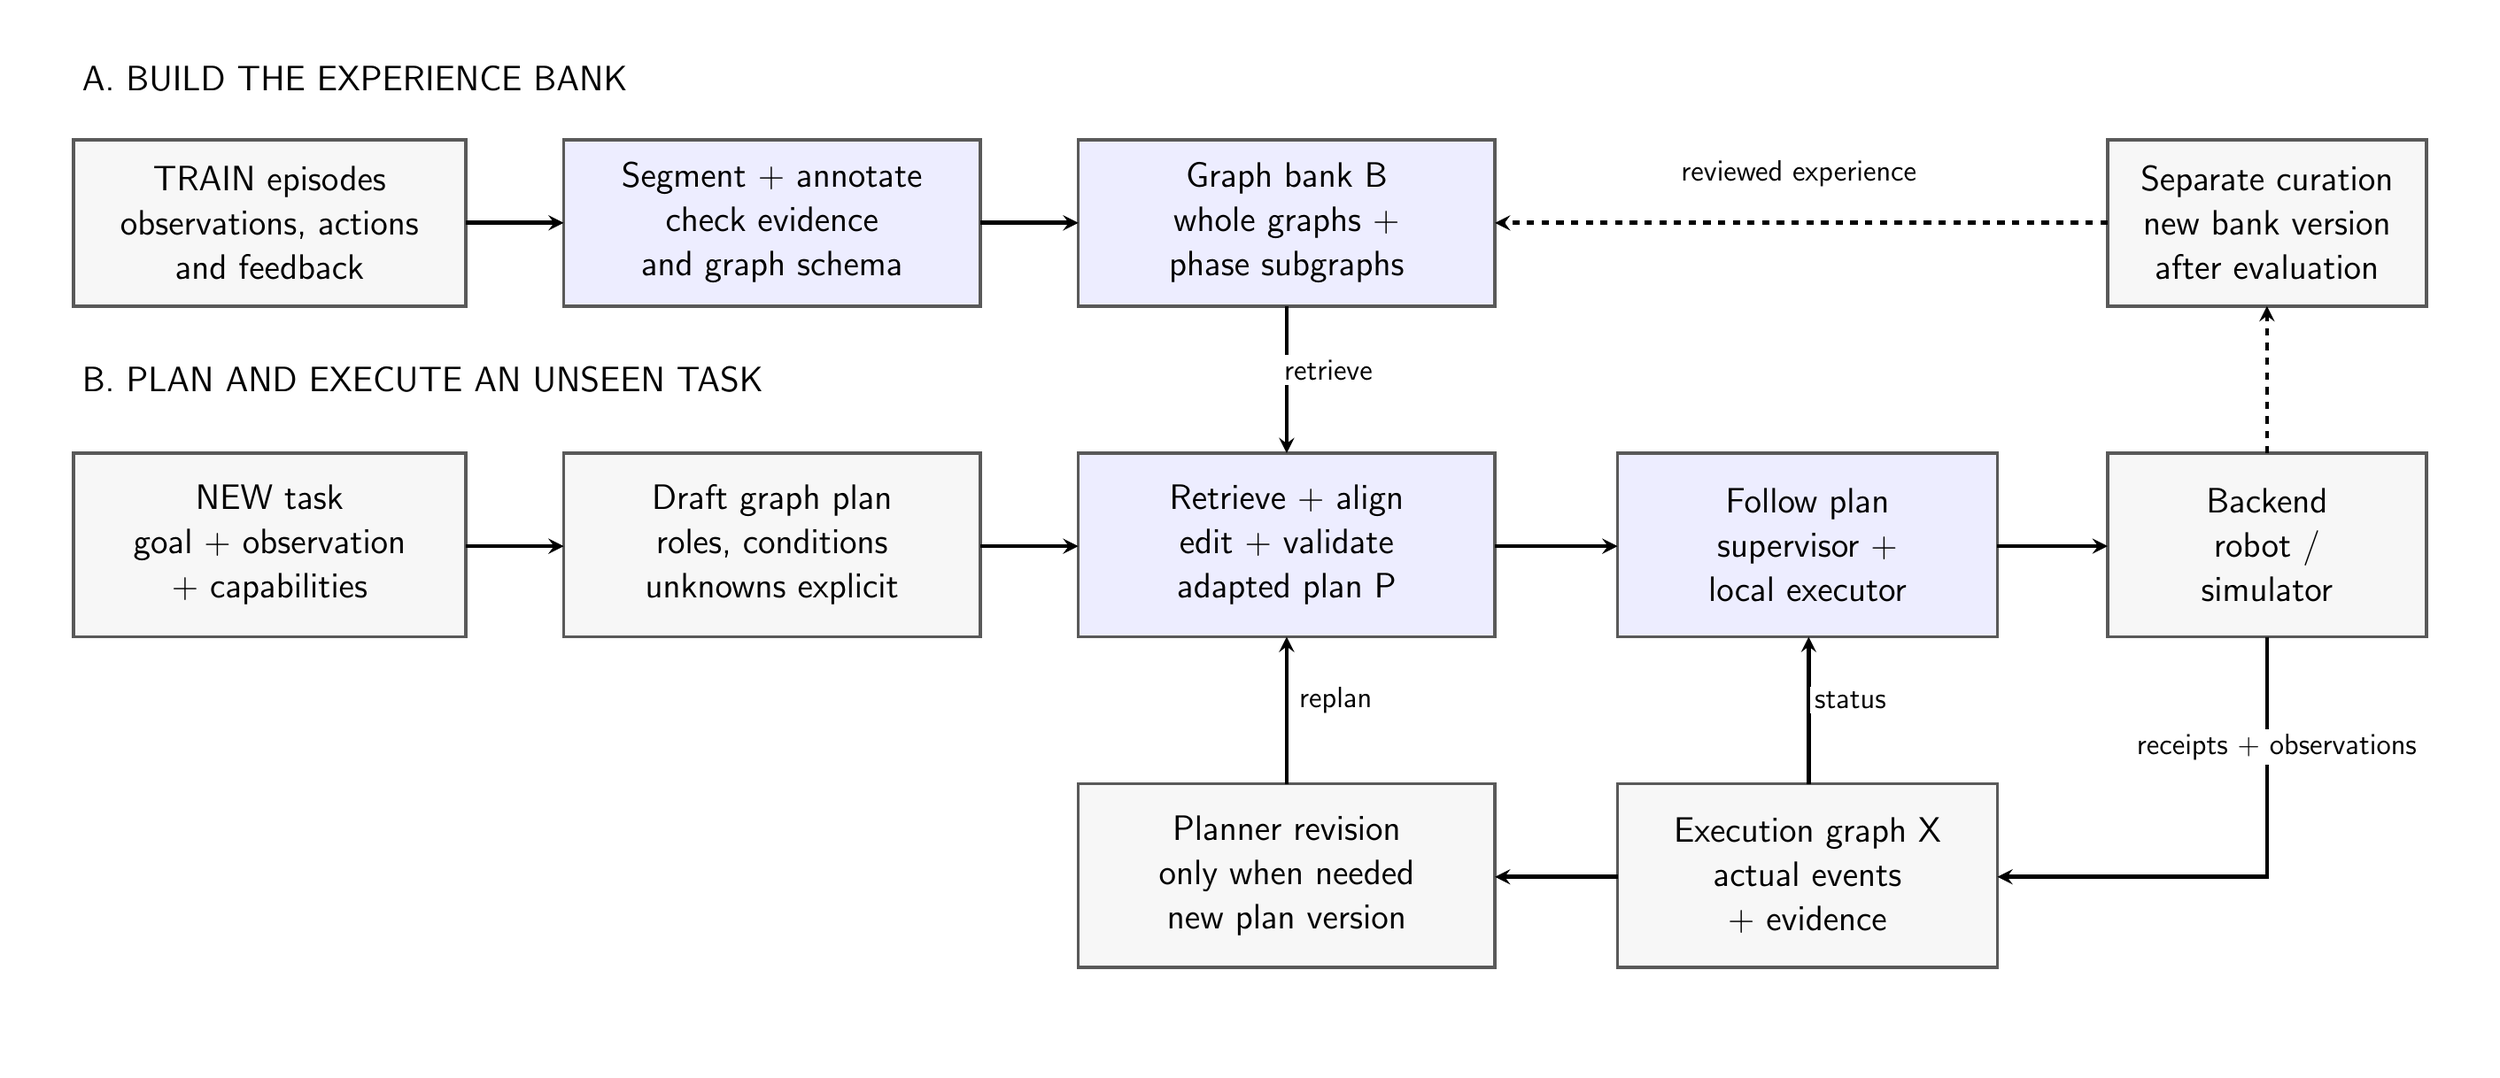
\begin{tikzpicture}[x=1pt,y=1pt,>=stealth]
\path[use as bounding box] (0,0) rectangle (1000,420);
\node[draw=black!65,fill=black!3,line width=1.3pt,minimum width=160pt,minimum height=68pt,text width=148pt,inner sep=4pt,align=center,font=\sffamily\fontsize{14}{18}\selectfont] (episodes) at (100.0,339.0) {TRAIN episodes\\observations, actions\\and feedback};
\node[draw=black!65,fill=blue!7,line width=1.3pt,minimum width=170pt,minimum height=68pt,text width=158pt,inner sep=4pt,align=center,font=\sffamily\fontsize{14}{18}\selectfont] (annotate) at (305.0,339.0) {Segment + annotate\\check evidence\\and graph schema};
\node[draw=black!65,fill=blue!7,line width=1.3pt,minimum width=170pt,minimum height=68pt,text width=158pt,inner sep=4pt,align=center,font=\sffamily\fontsize{14}{18}\selectfont] (bank) at (515.0,339.0) {Graph bank B\\whole graphs +\\phase subgraphs};
\node[draw=black!65,fill=black!3,line width=1.3pt,minimum width=160pt,minimum height=75pt,text width=148pt,inner sep=4pt,align=center,font=\sffamily\fontsize{14}{18}\selectfont] (input) at (100.0,207.5) {NEW task\\goal + observation\\+ capabilities};
\node[draw=black!65,fill=black!3,line width=1.3pt,minimum width=170pt,minimum height=75pt,text width=158pt,inner sep=4pt,align=center,font=\sffamily\fontsize{14}{18}\selectfont] (draft) at (305.0,207.5) {Draft graph plan\\roles, conditions\\unknowns explicit};
\node[draw=black!65,fill=blue!7,line width=1.3pt,minimum width=170pt,minimum height=75pt,text width=158pt,inner sep=4pt,align=center,font=\sffamily\fontsize{14}{18}\selectfont] (adapt) at (515.0,207.5) {Retrieve + align\\edit + validate\\adapted plan P};
\node[draw=black!65,fill=blue!7,line width=1.3pt,minimum width=155pt,minimum height=75pt,text width=143pt,inner sep=4pt,align=center,font=\sffamily\fontsize{14}{18}\selectfont] (follow) at (727.5,207.5) {Follow plan\\supervisor +\\local executor};
\node[draw=black!65,fill=black!3,line width=1.3pt,minimum width=130pt,minimum height=75pt,text width=118pt,inner sep=4pt,align=center,font=\sffamily\fontsize{14}{18}\selectfont] (world) at (915.0,207.5) {Backend\\robot /\\simulator};
\node[draw=black!65,fill=black!3,line width=1.3pt,minimum width=155pt,minimum height=75pt,text width=143pt,inner sep=4pt,align=center,font=\sffamily\fontsize{14}{18}\selectfont] (history) at (727.5,72.5) {Execution graph X\\actual events\\+ evidence};
\node[draw=black!65,fill=black!3,line width=1.3pt,minimum width=170pt,minimum height=75pt,text width=158pt,inner sep=4pt,align=center,font=\sffamily\fontsize{14}{18}\selectfont] (revise) at (515.0,72.5) {Planner revision\\only when needed\\new plan version};
\node[draw=black!65,fill=black!3,line width=1.3pt,minimum width=130pt,minimum height=68pt,text width=118pt,inner sep=4pt,align=center,font=\sffamily\fontsize{14}{18}\selectfont] (curate) at (915.0,339.0) {Separate curation\\new bank version\\after evaluation};
\draw[->,line width=1.7pt] (180,339) -- (220,339);
\draw[->,line width=1.7pt] (390,339) -- (430,339);
\draw[->,line width=1.7pt] (180,207) -- (220,207);
\draw[->,line width=1.7pt] (390,207) -- (430,207);
\draw[->,line width=1.7pt] (515,305) -- (515,245);
\node[fill=white,inner sep=2pt,font=\sffamily\fontsize{12}{14}\selectfont] at (532,279) {retrieve};
\draw[->,line width=1.7pt] (600,207) -- (650,207);
\draw[->,line width=1.7pt] (805,207) -- (850,207);
\draw[->,line width=1.7pt] (915,170) -- (915,72) -- (805,72);
\node[fill=white,inner sep=2pt,font=\sffamily\fontsize{12}{14}\selectfont] at (919,125) {receipts + observations};
\draw[->,line width=1.7pt] (650,72) -- (600,72);
\draw[->,line width=1.7pt] (515,110) -- (515,170);
\node[fill=white,inner sep=2pt,font=\sffamily\fontsize{12}{14}\selectfont] at (535,144) {replan};
\draw[->,line width=1.7pt] (728,110) -- (728,170);
\node[fill=white,inner sep=2pt,font=\sffamily\fontsize{12}{14}\selectfont] at (745,144) {status};
\draw[->,line width=1.7pt,dashed] (915,245) -- (915,305);
\draw[->,line width=1.7pt,dashed] (850,339) -- (600,339);
\node[fill=white,inner sep=2pt,font=\sffamily\fontsize{12}{14}\selectfont] at (724,359) {reviewed experience};
\node[anchor=base west,font=\sffamily\fontsize{15}{18}\selectfont] at (20,393) {A. BUILD THE EXPERIENCE BANK};
\node[anchor=base west,font=\sffamily\fontsize{15}{18}\selectfont] at (20,270) {B. PLAN AND EXECUTE AN UNSEEN TASK};
\end{tikzpicture}}
\caption{Proposed RoboRAG workflow. Training episodes are segmented and checked to form a versioned bank $\mathcal{B}$ of experience graphs $G$. A new goal, current observation and backend capabilities produce a draft plan $P$. Retrieved graphs or subgraphs supply phase structure, conditions and recovery evidence; alignment and validation produce an adapted plan. A supervisor follows approved phases through a local executor, while the planner handles structural revisions. Actual receipts and observations extend the execution graph $X$. The three graphs share a schema, but history, intent and observed execution retain distinct status. The training bank stays fixed during held-out evaluation; the dashed return path is used only by a separately evaluated curation process. This is a method diagram, not an experimental result.}
\label{fig:overview}
\end{figure*}
